\chapter{Brugersikkerhed} \label{sec:brugersikkerhed}
Når kroppen forbindes med et elektronisk system, opstår der en risiko for at påføre kroppen uønskede fysiologiske reaktioner ved at lade strøm passere gennem kroppen \citep{webster1998}. Disse fysiologiske reaktioner kan ses på \autoref{fig:makromikro}. 

\begin{figure}[H]
\centering
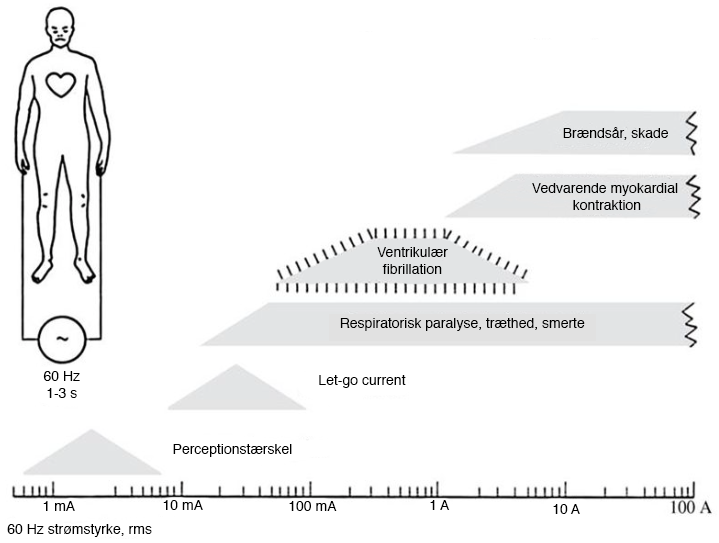
\includegraphics[width=1\textwidth]{figures/makromikro}
\caption{Når $60~Hz$ strøm går gennem hænderne i $1-3~s$, påvirkes en $70~kg$s person forskelligt alt efter, hvor stor en strømstyrke, personen udsættes for \citep{webster1998}.}
\label{fig:makromikro}
\end{figure}

\noindent
Kropsvægt og indgangssted for strømmen afgør, hvilken effekt strømmen har på brugeren. Alt efter, hvordan strømmen løber gennem kroppen og hjertet, kan der opstå mikro- eller makrochok. Hvis hjertet tilføres strøm direkte, og denne derefter går direkte til jord, er det mikrochok. Mikrochok kan ske, hvis en invasiv komponent placeres i direkte kontakt med hjertet. Hvis en person er tilkoblet strøm flere steder, kan der opstå makrochok, da en lille del af strømmen kan gå gennem hjertet. For at undgå makrochok, kan systemet benytte små spændinger og strømstyrke samt batterier for at frakoble personen elnettet \citep{webster1998}.

\section{Sikkerhedsforanstaltninger}
For at undgå mikro- og makrochok kan jording og isolation benyttes som sikkerhedsforanstaltninger. På denne måde kan brugerens sikkerhed opretholdes under brug af systemet. Jording og isolation kombineres ofte, da dette er den mest effektive metode til at sikre brugeren \citep{webster1998}.

\subsection{Jording}
Jording sikrer systemets bruger ved at benytte én fælles referenceværdi for alle systemets blokke. Jording beskytter på denne måde imod mikro- og makrochok, da strømmen vil blive ledt mod jord, ved fejl i kredsløbet. Strømmen afledes dermed fra systemets bruger \citep{webster1998}.

\subsection{Isolation}
Isolation sikrer systemets bruger ved at sørge for, at strøm i form af fejl- eller lækstrømme ikke løber fra én del af systemet til en anden, da dette kan medføre makrochok. Ved at isolere, er det dermed ikke muligt for fejl- eller lækstrømme at nå systemets bruger \citep{webster1998}. 

\section{Implementering af brugersikkerhed}
I dette system kombineres jording og isolation for at sikre systemets bruger mest effektivt. Systemet jordes ved at have en fælles jord for alle systemets komponenter - denne kommer fra spændingsforsyningens GND-terminaler, der er illustreret på \autoref{fig:spaendingsforsyning}. Isolation sikres ved at lade systemet være adskilt fra computeren, der benyttes til datavisualisering, ved brug af den trådløse BLE-forbindelse. Derudover adskilles systemet fra elnettet ved brug af batterier som spændingsforsyning. På denne måde kommer brugeren af systemet ikke i forbindelse med høje spændinger eller strømme. 

